%!TEX TS-program = xelatex
%!TEX encoding = UTF-8 Unicode
%

% Madrona Labs Aalto manual.
% XeLaTeX format.

% --------------------------------------------------------------------------------------------------------------------------------
% here are examples of how to set figures, notes and equations.

%\begin{marginfigure}
%	\includegraphics[width=\marginparwidth]{images/fig_1.pdf}
%	This manual is released under the Creative Commons Attribution 3.0
%	\caption{A caption}
%\end{marginfigure}

%\begin{figure}
%	\includegraphics[width=\textwidth]{aalto_screenshot.png} 
%	\caption{This figure lives happily within the text area.}
%	\label{fig:aalto}
%\end{figure}

%\begin{figure*}
%	\includegraphics[width=\textwidth]{aalto_screenshot.png} 
%	\caption{This figure juts out into both margins}
%	\label{fig:aalto2}
%\end{figure*}

%\marginnote{\textsc{Protip: }It is well known that the capacitance between a pair of parallel plate conductors varies inversely as the distance between the conductors.  This principle has been used to construct a variety of capacitive sensors.  Capacitive force sensors can be made using conductive layers separated by an elastic dielectric.}

%\begin{equation*}
%S_{n}(r) = 
%	 a_{m,n} 
%	 \left(
%	 	e^{ 2 \pi j \frac{k}{N}(m+c)}  + e^{-2 \pi j \frac{k}{N}(m+c)} 
%	\right)
%	e^{-2 \pi j \frac{k}{N}r} .
%\end{equation*}


%This is Chapter~\ref{ch:syn}. It starts on page~\pageref{ch:syn}.


% --------------------------------------------------------------------------------------------------------------------------------
% packages -- order is important!
\documentclass[nofonts, justified, marginnote=raggedright,  caption=raggedright]{tufte-book}	% gave up getting symmetric to work
\usepackage{arev}		% use arev font for math.
\usepackage{graphicx}
\usepackage{pdfpages}
\usepackage{amsmath}
\usepackage{color}
\usepackage{lipsum}	% for providing filler text
\usepackage{textpos}	%absolute positioning, for background pictures
\usepackage{fontspec}
\usepackage{leading}
\usepackage{fancyhdr}
\usepackage{sectsty}
\usepackage{xunicode}
\usepackage{makeidx}
\makeindex

% --------------------------------------------------------------------------------------------------------------------------------
% page dimensions

\usepackage{geometry}
\geometry{paperheight=7in, paperwidth=7in }
%\geometry{height=6in, width=6in }
\geometry{includeall}
\geometry{left=0.5in, textwidth=3.75in, marginparsep=0.25in, marginparwidth=2in}
\geometry{top=0.25in, headheight=0.25in, headsep=0.125in, footskip=0.5in, textheight=5.5in}
%\geometry{twoside} % gave up getting this to work with tufte-book


% --------------------------------------------------------------------------------------------------------------------------------
% numbering


 \setcounter{secnumdepth}{-1}


% --------------------------------------------------------------------------------------------------------------------------------
% colors
\definecolor{textC}{cmyk}{0, 0, 0, 1} 
\definecolor{darkC}{cmyk}{0., 0.60, 1.0, 0.79} 
\definecolor{lightC}{cmyk}{0., 0.33, 0.61, 0.18} 
\definecolor{bgC}{cmyk}{0.0,0.0,0.00,0.} 

\def\headingcolor

% --------------------------------------------------------------------------------------------------------------------------------
% fonts  -

% idiocy: pdflatex version is required to use the microtype package and get optical justification.
% set tex Program to pdftex / pdflatex in Prefs./Misc./Personal Script to enable.
%\usepackage[expansion=false,protrusion=true,final]{microtype}

\defaultfontfeatures{Mapping=tex-text}

\setmainfont{Minion Pro}

\newfontfamily\madronalogofont{FontinSans-SmallCaps}

\newfontfamily\madronachapfont{MadronaSans-CondensedOblique}

\chapterfont{\madronachapfont\huge\leading{24pt}\color{lightC}\addfontfeature{LetterSpace=0.0}}                 
 
\setcaptionfont{\setmainfont {MinionPro-MediumIt}  \footnotesize}

% example of adding to commands 
%\let \oldcaption \caption
%\renewcommand{\caption}{\color{lightC} \oldcaption}

% --------------------------------------------------------------------------------------------------------------------------------
% Madrona Labs definitions

\usepackage{relsize}

\newcommand{\ctrl}[1]{{\relsize{-0.5}\madronachapfont\addfontfeature{LetterSpace=2.0}{#1}}}

\newcommand{\module}[1]{{\madronachapfont \smaller \uppercase{\emph{#1}}}}

\newcommand{\URL}[1]{{\madronachapfont \smaller {\emph{#1}}}}

%\newcommand{\illo}[1]{\marginnote{ \madronachapfont \larger \color{lightC} ILLO: #1}}
\newcommand{\illo}[1]{}

%\newcommand{\patch}[1]{{\relsize{-0.5}\madronachapfont\addfontfeature{LetterSpace=0}\emph{#1}}}
%\newcommand{\patch}[1]{\emph{#1}}
\newcommand{\patch}[1]{“{#1}”}


\let \oldsection \section
\renewcommand{\section}[1]{\oldsection{\textnormal{#1}}}

%\newcommand{\colorsection}[1]{\section{\color{lightC}#1}}
\newcommand{\colorsection}[1]{\section{\larger{#1}}}

\let \oldsubsection \subsection
\renewcommand{\subsection}[1]{\oldsubsection{\textnormal{{#1}}}}



\newcommand{\question}[1]{{\vskip 0.5em\noindent{\emph{#1}}}\vskip 0.25em}

\newcommand{\answer}[1]{{\noindent{#1}}\vskip 1em}




% --------------------------------------------------------------------------------------------------------------------------------
% chapter header

% Format the chapter headings 
\makeatletter 
\titleformat{\chapter}% 
  [block] % shape arg
  {\relax\ifthenelse{\NOT\boolean{@tufte@symmetric}}{\begin{fullwidth}}{}} % format applied to label+text 
  {\huge \madronachapfont \addfontfeature{LetterSpace=-2.0} \color{lightC}\thechapter\quad} % label 
  {0pt} % horizontal separation between label and title body 
  {\huge \madronachapfont \addfontfeature{LetterSpace=-2.0} \color{lightC}} % before the title body 
  [\ifthenelse{\NOT\boolean{@tufte@symmetric}}{\end{fullwidth}}{}]

% after the title body 
\makeatother 

% --------------------------------------------------------------------------------------------------------------------------------
% document headers and footers

\pagestyle{fancy}
\fancyhead{} % clear all header fields 
\fancyfoot{} % clear all footer fields 
\fancyfoot[LE,RO]{\thepage} % add page number


% --------------------------------------------------------------------------------------------------------------------------------
% document

\begin{document}

% --------------------------------------------------------------------------------------------------------------------------------
% document tolerance

\pretolerance=-1
\tolerance=2300
\adjdemerits=6400
\doublehyphendemerits=90000
\finalhyphendemerits=14400
\widowpenalty=3000
\clubpenalty=3000

% --------------------------------------------------------------------------------------------------------------------------------
% document colors

\pagecolor{bgC}
\color{textC}

% --------------------------------------------------------------------------------------------------------------------------------
%  title page
% requires \usepackage{pdfpages}

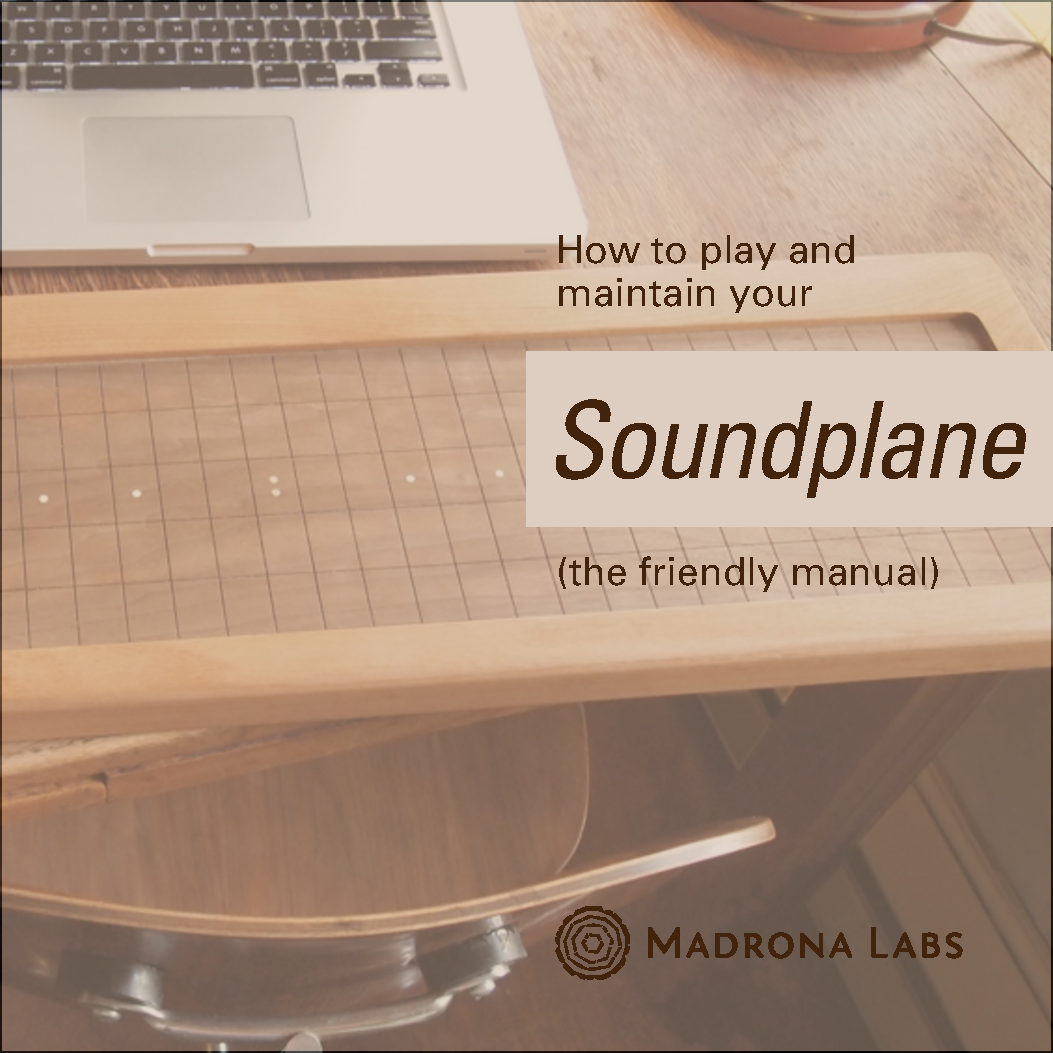
\includepdf{images/SoundplaneManualCover.pdf}

% --------------------------------------------------------------------------------------------------------------------------------
%license and colophon page


\thispagestyle{empty}
{
\raggedright
\ \ \vskip 2in
\noindent 
This manual is released under the Creative Commons Attribution 3.0 Unported License.  You may copy, distribute, transmit and adapt it, for any purpose, provided you include the following attribution: \\
{\itshape Soundplane and the Soundplane manual by Madrona Labs. 
http://madronalabs.com.}

\vspace{1 em}
\noindent 
Version 0.9, June 2012.  Written by Randy Jones.

\vspace{1 em}
\noindent 
%Illustrated by David Chandler.

\vspace{1 em}
\noindent 
Typeset in Adobe Minion using the \TeX \ document processing system. 

\vspace{1 em}
Any trademarks mentioned are the sole property of their respective owners.  Such mention does not imply any endorsement of or association with Madrona Labs. 
}


% --------------------------------------------------------------------------------------------------------------------------------



%
\chapter{QUICK START}
%could go here. 

To enjoy your Soundplane, the very first thing to do is visit the forums at madronalabs.com for the latest client software and example patches.  These will be updated every week or so for the near future.  

\begin{itemize}
\item Visit the hardware forum at madronalabs.com.
\item Plug in your Soundplane using any A->B USB cable.
\item Download and run the Soundplane client application. 
\item The Soundplane will automatically calibrate for a few seconds.  Keep hands and other objects away from the surface during this time.
\item Now touch the surface and you should see the touches in the grid view.
\item Click the right arrow to go to the Output page. Here you see the options for OSC and MIDI output.  Dive in and experiment for a bit, or read on to learn more. 

\end{itemize}


%still no numbering
\chapter{Introduction}

First, a heartfelt thanks to all of you intrepid Soundplane owners, whose support and whose patience made building this new instrument possible. 

Second, congratulations on your purchase.  Based on a solid foundation in open research, and made with a consistent devotion to both technical and aesthetic details, the Soundplane is one of the most intimate and expressive interfaces for computer music available at any price.  We hope that it inspires you and opens up new worlds of sonic expression for you. 

This is an early draft of the Soundplane manual which will be updated often.  I'm going to put all my notes into this document and gradually shape them up in order to get the information out as quickly as possible.  In other words, ”under construction”—thanks for your understanding. 


% turn on numbering for parts and chapters 
\setcounter{secnumdepth}{0}

\chapter{The hardware}

Simplicity was a main design goal for the Soundplane. so a tour of the hardware is quick.  The alder body looks great and holds everything in place.  The aluminum bottom and back panel allow the instrument to be lighter and thinner than wood alone would.  The USB jack provides both data transport and power.  Because the Soundplane runs on a custom, low-power DSP board, any laptop computer should be able to provide sufficient current.

On the front is a power light with a walnut surround.  This light goes on when contact with the Soundplane has been established by its client software.  It doesn't go on if the software is not running.  

\section{The surface}

The Soundplane’s playing surface is a hybrid between a keyed instrument like a piano, and a fretless instrument like a violin, equally playable in either mode with the right software.  It's a uniquely flexible setup but also potentially confusing.  The top of the surface is divided into 150 keys in five rows of 30, 13 of them with inlaid fret markings that serve as visual cues for orienting your fingers.  The Soundplane can send out a different MIDI note or OSC message for each key.  

The keys are very thin, and attached to a thick piece of rubber that allows each one a small amount of independent motion.  Under the rubber is a continuous sensing surface that detects the applied pressure at a higher resolution than the keys, 64 by 8 sensing elements.  By calculating the centroids of pressure data, the positions of applied touches can be calculated to a resolution much finer than the sensor grid.  

\section{Setup}

The Soundplane senses all the forces applied to its surface, including gravity and the acceleration of the whole instrument, and the playing context needs to be set up with this in mind.  Designed to be played lying flat on a fixed surface such as a table, with its six little rubber feet (LRFs) in contact with the surface, is how it will be most sensitive.  

However, the dynamic software calibration also attempts to separate finger pressure from pressure due to gravity or motion.  So, it’s possible to play in other orientations besides the horizontal, or on an unstable surface like one’s lap.  It's probably best to learn basic techniques on a flat surface and then experiment with other playing positions. 

\section{Break in and first playing}

The Soundplane's surface needs to lie flat against its internal sensors in order to have a consistent response.  After being moved significantly, such as in shipping, the surface may ride up on its supports a bit.  So, after any major motion and before playing, I recommend a short break-in to get the response consistent.  Press all over the surface with a kneading motion, like a massage.  Just ten seconds or so should be enough.  Then press the recalibrate button in the Soundplane application to lock in the new rest position. 

This break-in process will make the response more uniform across the surface.  I have also found that as the rubber stretches and wears over time, the response becomes gradually more uniform. 

The break-in massage is purely mechanical and can be done without the Soundplane plugged in.  

Plug in a USB cable and launch the Soundplane client application to begin playing.  

\section{How it works, briefly}

The Soundplane is a capacitive sensor, but unlike inflexible touchscreen sensors, it doesn't measure capacitance between your hand and a fixed surface.  Instead, it measures capacitance between two sets of internal plates, one fixed and one that you move by pressing on the surface.  One advantage of this approach is that you get tactile feedback because you are actually moving a sensor element through space.  It's a small amount of motion, around 1mm, but it makes a big difference in how the instrument feels as opposed to a solid glass surface.  Another advantage is that anything that can press on the surface can be used to play.  I have had good luck with soft yarn mallets. 

\chapter{The software}

The USB specification defines certain device classes, which allow some pieces of hardware to be recognized without any special software.  Some of these are printers, audio interfaces, and mass storage devices.  But none of these were really sufficient to convey all the data that Soundplane has to offer.  So we wrote a custom software application, the Soundplane client, that reads raw pressure data and translates it into OSC (Open Sound Control) and MIDI data.   

When first launched, the application's window appears in the center of the main monitor. When moved, the window's location will be remembered the next time the application is launched. 

\section{Calibrating}

When first launched, the client shows the Touches page and calibrates the Soundplane by grabbing pressure readings and averaging these over several seconds.  This is just like taring (zeroing) a scale—but with 512 scales, one for each of the Soundplane’s sensing elements!  During calibration a progress bar is shown.  \emph{Do not touch the surface during this time!}  Pressing the recalibrate button at any time will clear the current touches and redo this process. 

\section{Preset menu}

On top is a preset button marked “continuous pitch x” that currently does nothing.  Nothing!  This is where configuration presets will be stored.  Right now (v. 0.9) the app does not remember any of its configuration.  

\section{Grid view}

On the top, this is where the pressure data can be viewed, as raw data directly from the sensors, calibrated data, or recognized touches (cooked).  the menu in the lower right selects these modes.  

\section{Touch view}

Under the grid view is the touch timeline view, showing a short history of pressure data for each touch.  

The \ctrl{touches}  dial sets the maximum number of possible touches.  If more touches are applied to the surface, the touches with the greatest force will be selected. 

Setting \ctrl{touches}  to 1 will give this view the most resolution.

The \ctrl{thresh} dial sets the force required to activate a touch.  The default of 0.020 is quite conservative, and should not result in any false touches.  Bringing this value down will make the instrument more sensitive.

The \ctrl{max force} dial sets the maximum absolute force that will be output.  

The \ctrl{z curve} dial, just like on MIDI performance keyboards, sets the curve that will be applied to the touch pressure data between the sensors and the data output.  The results of this control can be seen in the touch timeline. 

\section{The footer}

The footer is where the device serial number, firmware version and status are shown. 

In addition there's a resize widget on the lower right.  Dragging it resizes and scales the whole interface.  

\section{Zones page}

Clicking the right/left arrows changes from one page in the app to another.  To the right of the Touches page is the Zones page.  

The big display area does nothing yet. Here you will be able to turn all of the keys into different zones for notes or controllers as soon as I finish writing that software. 

The \ctrl{data freq} dial controls how many times per second the Soundplane client outputs MIDI and OSC data.  Note-ons (and their equivalents over OSC) will always be output ASAP, but everything else (x, y and pressure for each touch) will only be sent at this frequency. 

MIDI area: pick a MIDI device, or turn MIDI on / off entirely.

OSC area: turn OSC on / off entirely.  The accompanying Max/MSP patch shows how to receive OSC data.  Always sent on port 3123 for now.  The OSC data are sent in the very compact t3d format, a subset of the TUIO2 format invented for multi-touch devices.  

Zones output note numbers, not pitches.  It's up to any application that receives the MIDI or OSC data to decide what pitches to play. 

The note number can be fractional-- the behavior of the fraction will be set by the quantize or "snap" control.  With no quantize the note number is always a bilinear interpolation from position to the surrounding note values.  With full quantize, the note number is always an integer, the number of the note the touch is in.  In between, the number drifts towards the integer values with a variable time scale.  Like Autotune actually.



\section{Expert page}

Another page with some dials you may not want to mess with. A work in progress. 


\section{Working with sound engines}

FROM CONTINUUM 
Generally you should use synthesis algorithms that have dynamics controlled by channel pressure or a continuous controller (like expression, volume, or breath). Avoid using Note On key velocity to control dynamics. While the Continuum Fingerboard can be configured to transmit Note On key velocity, it is not usually recommended. Key velocity is a single discrete value that is determined on the note’s attack but affects the entire note, unlike a continuous controller which can constantly output a stream of data while a note is sounding. For instance, if you were to use key velocity to affect note volume, you could not start a note quietly and then swell to a loud dynamic during the note's duration. This is the reason the Continuum Fingerboard (like Midi breath controllers) defaults to transmitting a constant 127 for key velocity, and does all dynamic control using channel controllers.
Finally, avoid synthesis algorithms that trigger amplitude envelopes on Note On. An apparent ‘double trigger’ or ‘stutter’ effect can result: first you hear the amplitude envelope that is triggered when the finger comes in contact with the playing surface, then you hear a second amplitude increase as the performer’s finger pressure increases on the playing surface. In most cases only the performer's finger pressure variations should be controlling the amplitude, not a built-in envelope. However, if you find that the sound uses an amplitude envelope that you like and don’t want to discard, consider mapping pressure into another controller that does not affect amplitude.

When using an external synthesizer, it is important to verify proper Pitch Bend Range configuration: Play a glissando; when you lift your finger at the end of the glissando, play a new note at the spot where you lifted your finger. The pitch at the end of the glissando should match the new note’s pitch; if not, the Pitch Bend Range configured on your Continuum Fingerboard does not correctly match your synthesizer.

y default cc 74
z default cc 11
cc 96 for kyma pitch bend range?!


\chapter{Putting it together}


\section{Playing technique}

DRAFT 

The Soundplane is an instrument capable of supporting a wide range of expressive gestures.  As with any instrument, practice is needed to get to the stuff you are really after.  Intentionality is key.  Because you are able to play notes that go wandering... if your fingers wander that’s what you’ll get.  To play crisp, decisive notes you will need a crisp, decisive touch.


Threshold : sensitivity vs. position / false touches.  A tradeoff.  Light touches are less definite as to position. A harder touch will track a finger more accurately and lighter touches may wander more.



\section{Hysteresis}

Since the Surface takes some time to return to its resting state after a finger’s pressure is removed, a smaller threshold will also increase the release time for touches, making them linger more after a finger is released. 

Likewise, a very hard touch will always take a lot longer to return to the resting state.  You can set the \ctrl{max force}  dial to get the tradeoff between response and firmness you want. 

We recommend you get to know your Soundplane using the default threshold of 0.02, which is a light but definitely intentional touch.  You can then reduce the threshold as your own taste dictates, and your radio frequency noise environment permits.  

\section{Proximity}

At 64 by 8 sensing elements, the sensor grid is twice the resolution of the Soundplane’s keys in the x dimension, and less than twice in the y dimension.  Since each touch of a finger affects quite a few sensing elements around it, there is a limit to how close two finger touches can get and still be seen by the Soundplane as separate.  

Two fingers should always be seen as separate if there is one key or more in between them.  If two fingers are on adjacent keys, they will be seen as one touch, unless the layer takes great care to place them as far apart as possible on the two keys, in two opposite corners.  

If you want to play lots of close intervals, this can be done in at least two ways.  If each row has a different starting pitch, then there can be zones several keys away from each other that have the same pitch.  Then unisons or minor seconds (adjacent notes) can be played in the way they are on a guitar. 

On the other hand, if the zones are set up so that each row has the same pitch, then close intervals can be played on adjacent columns, but separated vertically from each other.  

 

\section{Touch speed and dynamic calibration}


The Soundplane dynamically calibrates all of the areas on its surface that are not currently being touched, by collecting the current pressure data through a very slow filter and setting the result as the new zero reference.   This approach does a good job of eliminating long-term shifts in the force values like the changes when the Soundplane is tilted.  It means ,however, that any touch applied more slowly than the filter's response speed will be itself regarded as background noise.  This speed is about equal to a ten second movement from no pressure to the heaviest possible pressure—a very slow touch.  It's possible to fool the filter, but you need a very steady hand and the intent to do so.  

The Soundplane is playable with many objects, but the software is optimized for detecting finger touches.  You could try soft mallets. 
 

The soundplane's surface is calibrated dynamically to separate forces due to gravity.  This calibration nulls out slow changes in the data while allowing quicker changes, such as touches, to pass through.  It means, however, that there is a slowness threshold under which a touch will be interpreted as background noise.  It's kind of like sneaking past a motion detector: if you press down very very slowly on the surface, your touch will not appear.  Any more typical musical gesture, though, even down to a \emph{pppp,} should be recognized.


\chapter{Care and feeding}

The Soundplane is built more like a fine acoustic instrument than a plastic MIDI keyboard.  That's part of why you're here.  But having such a nice organic form factor comes with the need for a bit of mindful care.  

First of all, the walnut veneer surface is more delicate than a plastic keyboard.  Hard playing with the fingers and hands is definitely considered normal use.  However, nails can leave small marks in the surface and if you contact one of the veneer edges fairly hard wiht a nail it's possible to chip off a bit of wood.  Keeping the fingernails trimmed is probably best.  

Also, like a guitar, the wooden body moves with changes in temperature and humidity.  Though the structure is made with this in mind, extremes of humidity may still cause a small amount of warping that affects playability.  

The alder body is finished with ProFin, a permanent polymerized oil finish made by the Daly’s company in Seattle.  Over this is a coat of furniture wax for durability.  If the wax eventually becomes dull due to handling, repair with any standard furniture wax is possible.  We use “Black Bison” from Liberon.  

The walnut playing surface is finished with a product called Howard’s Butcher Block conditioner.  This is just wax and mineral spirits and is food-safe.  If the surface becomes too dull or dry, rub on a small amount of this or any butcher block finish, wait 5–10 minutes for it to dry and wipe off the excess with a clean soft cloth.  Start with just a few drops and add more oil as needed—you don't want to over-oil it.  

For oiling cutting boards the saying is ”once every day for a week, once every week for a month, and once a month forever.”  This might also apply to Soundplanes.  How oily you want to keep the surface is a matter of taste.  

Excess oil, as well as dust, crumbs, etc, may get into the cracks between keys.  Though they don't really do any harm, they can be unsightly.  An African porcupine quill is an ideal tool from removing them.  If you don't have a porcupine quill, a sharp stick works too.  Sharp metal is not recommended due to the danger of scratching the surface. 


\appendix

\chapter{Frequently asked questions}

If the application window is ever missing when launched, it may be remembering its position on an external monitor that is not currently connected. To reset the window setting, launch the Soundplane app while holding the Command key. 


\question{Question
}
\answer{Answer
}


\printindex

\end{document}


